\documentclass{article}
\usepackage{amsfonts}          % Para las negrita de pizarra
\usepackage{indentfirst}       % Para que quede mas lindo el formateo
\usepackage{graphicx}          % Para graficos
\usepackage{minted}            % Para poner codigo y que quede con sintaxis fachera
\usepackage{hyperref}          % Para meter hipervinculos
\usepackage[dvipsnames]{xcolor}% Para usar colores
\usepackage{hhline}            % Mas configuracion para las líneas en tablas
\usepackage{amsmath}           % Agregado para tags de ecuaciones
\usepackage{xcolor}            % Coloreado de ecuaciones
\usepackage{quoting, xparse}   % Usado para citar
% \usepackage{svg}               % Para usar imagenes svg que se ven lindas independientemente del zoom. WARNING REQUIERE DE INKSCAPE. Tal vez no vale la pena
\usepackage{amsmath}

\graphicspath{ {./images/} }

\newcommand{\docuPy}{%
  {\href{https://wiki.python.org/moin/TimeComplexity}{documentacion oficial}}
  }%

  % Comandos para facilitar el citado
  % Fuente: https://tex.stackexchange.com/a/391739/273865
\NewDocumentCommand{\bywhom}{m}{% the Bourbaki trick
  {\nobreak\hfill\penalty50\hskip1em\null\nobreak
   \hfill\mbox{\normalfont(#1)}%
   \parfillskip=0pt \finalhyphendemerits=0 \par}%
}

\begin{document}

\begin{titlepage}
  \vspace*{1cm}

  \begin{center}
    {\Huge{Trabajo Práctico 3: Problemas NP-Completos para la defensa de la Tribu del Agua}}
  \end{center}

  \vspace{0.4cm}

  \begin{center}
    {\LARGE{Facultad de Ingeniería de la Universidad de Buenos Aires}}\\
    \vspace{0.3cm}
    {\Large{Teoría de Algoritmos}}\\
    \vspace{0.3cm}
    {\large{Cátedra Buchwald-Genender}}\\
  \end{center}

  \vspace{0.8cm}
  \begin{center}
    
\includegraphics[scale=0.8]{Logo-fiuba}
  \end{center}

  \vspace{1.4cm}
  \begin{center}

    {\begin{minipage}[t]{.32\textwidth}
        \begin{center}
          Gómez Belis, Sofía\\
          {\small{Padrón: 109358}}\\
          {\small{email: sgomezb@fi.uba.ar}}
        \end{center}
          \end{minipage}
          \begin{minipage}[t]{.32\textwidth}
        \begin{center}
          Llanos Pontaut, Valentina\\
          {\small{Padrón: 104413}}\\
          {\small{email: vllanos@fi.uba.ar}}\\
        \end{center}
      \end{minipage}
      \begin{minipage}[t]{.32\textwidth}
        \begin{center}
          Orsi, Tomas Fabrizio\\
          {\small{Padrón: 109735}}\\
          {\small{email: torsi@fi.uba.ar}}
        \end{center}
      \end{minipage}}

  \end{center}
\end{titlepage}

\renewcommand*\contentsname{Indice}
\tableofcontents
\pagebreak

\section{Introducción}
\subsection{Descripción y objetivo}

Continuando con el ataque de la Nación del Fuego sobre el resto de las naciones, esta vez es la Tribu del Agua la que requiere de nuestra ayuda para defenderse. 

Cada maestro agua tiene una fuerza o habilidad positiva $x_i$, y contamos con el conjunto de todos los valores $(x_i, x_2, \dots, x_n)$. Basándonos en estos, el maestro Pakku desea separar los maestros en \texttt{k} grupos $(S_1, S_2, \dots, S_k)$ parejos tal que cuando un grupo se canse, entrará el siguiente en el combate, obteniendo un ataque constante que les permita salir victoriosos, aprovechando también la ventaja del agua por sobre el fuego.

Para que los grupos estén lo más parejos posibles, nos han encomendado minimizar la adición de los cuadrados de las sumas de las fuerzas de los grupos:

$$
\min \sum_{i=1}^{k} \left( \sum_{x_j \in S_i} x_j \right)^2
$$

En este trabajo desarrollaremos algoritmos de backtracking, programación lineal y posibles aproximaciones buscando resolver el problema de optimización planteado con el objetivo de ayudar a los mestros de la Tribu del Agua a derrotar a la Nación del Fuego. También nos dedicaremos a demostrar que el problema de la tribu del agua es NP-Completo.

\section{Demostración de problema NP-Completo}
\subsection{Problema NP}
\subsection{Reducción}

\section{Complejidad algorítmica}

El problema de optimización de la tribu del agua fue resuelto utilizando distintas técnicas de programación. En las próximas secciones presentaremos el código correspondiente y analizaremos la complejidad temporal de cada uno de los algoritmos planteados:
\begin{itemize}
    \item Backtracking
    \item Programación Lineal
    \item Aproximación propuesta por la cátedra
    \item Aproximación adicional
\end{itemize}

\subsection{Complejidad lectura de archivos}
A continuación mostramos la función principal de lectura de archivos. 
\inputminted[linenos, firstline=9, lastline=24]{python}{codigo/archivos.py}

La función lee la línea que contiene la cantidad de conjuntos de maestros a crear. Una vez hecho eso, lee $n$ líneas para almacenar los distintos valores $x_i$ de tuplas (nombre, habilidad). Esto tiene una complejidad temporal $O(n)$.

\subsection{Complejidad algoritmo de Backtracking}

Debido al alto tiempo de ejecución de nuestro algoritmo inicial de backtracking, buscamos alternativas que nos permitieran disminuirlo. Logramos realizar algunas mejoras, las cuales serán analizadas en \nameref{sec:bt-greedy}. En ambos casos se realiza una poda cuando el algoritmo se da cuenta que la solución parcial no sirve. Esto ocurre cuando se hace una asignación de un maestro a un grupo que implica una suma mayor o igual a nuestra suma óptima. Cuando se da esta situación, se corta y se intenta asignarlo a otro grupo. Presentaremos a continuación ambas versiones del algoritmo. 

\subsubsection{Backtracking inicial}
Este algoritmo de bactracking utiliza la siguiente función auxiliar para calcular la adición de los cuadrados de la suma de las habilidades de cada grupo:
\inputminted[linenos, firstline=47, lastline=54]{python}{codigo/backtracking.py}

Esta función recorre los $k$ grupos para calcular la suma pedida. En el peor caso, la cantidad de maestros de un grupo puede ser $n$ (con $k = 1$), por lo que tiene un costo proporcional a $n \cdot k$. Diremos entonces, que la complejidad temporal de esta porción de código es $O(n \cdot k)$, con $k \leq n$ puesto que si $k > n$, nuestro algoritmo completo se ejecuta en $O(1)$.  

A continuación mostramos otras funciones que utiliza el código principal:

\inputminted[linenos, firstline=56, lastline=73]{python}{codigo/backtracking.py}

Como sabemos que si $n = k$ cada grupo tendrá únicamente un maestro, decidimos que en ese caso particular no se aplique el algoritmo de backtracking. En su lugar, resolvemos la asignación con la función \texttt{caso\_k\_igual\_a\_n} que itera sobre la lista de maestros, implicando un costo de $O(n)$. Esto nos permitió disminuir notablemente el tiempo de ejecución cuando $n = k$. 

Por otro lado, como necesitamos la habilidad de cada maestro para poder minimizar la función objetivo, nuestro algoritmo tiene en cuenta grupos con el nombre y la fuerza de cada maestro. Luego los filtramos para quedarnos únicamente con los nombres. Éste es el objetivo de \texttt{obtener\_resultado}. Su complejidad temporal es $O(n \cdot k)$, debido al mismo análisis que el de la función \texttt{sumatoria}.

Analizaremos ahora el código principal:
\inputminted[linenos, firstline=1, lastline=45]{python}{codigo/backtracking.py}

S $k > n$ no existe solución y si $k = 0$ no podemos formar grupos. En ambos casos el algoritmo funciona en $O(1)$. Sin embargo, se tratan de casos particulares. Procederemos a explicar el caso general.

En la \texttt{línea 14} ordenamos el conjunto de maestros por mayor habilidad con el algoritmo \href{https://svn.python.org/projects/python/trunk/Objects/listsort.txt}{Timsort} cuya complejidad es $O(n \cdot log(n))$, siendo $n$ la cantidad de maestros de la tribu que se enfrentarán a la Nación del Fuego. Crear los grupos vacíos en la línea \texttt{línea 13} es una operación lineal en la cantidad de grupos $k$, es decir, $O(k)$. 

La solución del problema viene dada por la función recursiva \texttt{problema\_tribu\
\_del\_agua\_bt\_recur}. Su objetivo es probar todas las combinaciones de asignaciones de maestros a los grupos de forma tal de minimizar la adición de los cuadrados de la suma de las habilidades de cada uno. Para cada maestro comprueba si, al asignarlo al grupo $i \in [0, k-1]$, se puede obtener una combinación con una suma menor a la actual. Caso contrario, poda y prueba con el si-\ guiente grupo. Iniciamos con una suma con valor infinito. La cantidad de posibles asignaciones es $k^n$ pues para cada uno de los $n$ maestros hay $k$ opciones de grupos. Por lo tanto, la complejidad de esta función y del algoritmo en general es exponencial, más específicamente $O(k^n)$.

\subsubsection{Backtracking - Greedy}
\label{sec:bt-greedy}

\inputminted[linenos, firstline=3, lastline=27]{python}{codigo/backtracking_con_greedy.py}

Esta función pública es bastante similar a la del algoritmo original, con la excepción de crear una lista de tamaño $k$, \texttt{sumas\_grupos}, cuyo costo es lineal.

Ambas versiones ordenan los maestros por mayor habilidad. Observamos que ésto mejoró el tiempo de ejecución. No es greedy, pero es una optimización. Para este caso decidimos seguir con una lógica similar, agregando otra optimización basada en el algoritmo de aproximación greedy propuesto por la cátedra. Éste consiste en asignar los maestros iterativamente en orden según su fuerza al grupo con la menor fuerza total hasta el momento. Se empieza por los más habilidosos. Utilizamos la misma idea para que cuando el algoritmo de backtracking intente agregar a un maestro a un grupo, lo haga en el grupo con menor habilidad. Si ésta no es una opción válida, continuamos con el siguiente grupo con menor fuerza. Ésto lo logramos ordenando los grupos. Como optimización adicional, guardamos en una lista la suma actual de cada grupo con el objetivo de evitar calcularlas en cada paso. La ordenamos en conjunto con los grupos usando \href{https://svn.python.org/projects/python/trunk/Objects/listsort.txt}{Timsort}, con un costo $O(k \cdot log(k))$.  

\inputminted[linenos, firstline=29, lastline=64]{python}{codigo/backtracking_con_greedy.py}

El algoritmo sigue realizando una búsqueda explícita del espacio de soluciones, por lo que su complejidad temporal es exponencial. Sin embargo, las mejoras nos permitieron reducir notablemente el tiempo de ejecución. Esto se debe a que se asigna rápidamente un maestro a un grupo con una suma pequeña, lo cual puede conducir a futuras podas (no se encuentra una suma mayor a la mejor hasta el momento). La comparación con el algoritmo original puede encontrarse en \nameref{sec:medidas-bt-greedy}. 
\subsection{Complejidad algoritmo de Programación Lineal}
\subsection{Complejidad algoritmo de Aproximación}

\subsection{Efecto de las variables sobre el algoritmo}

\section{Ejemplos de ejecución}
\label{sec:ejemplos}

En la carpeta \texttt{ejemplos\_adicionales} se pueden encontrar distintos casos de prueba que agregamos con el objetivo de comprobar la correctitud de los algoritmos propuestos. A continuación detallamos cada uno:
\begin{itemize}
    \item \texttt{uno\_por\_grupo.txt} $\rightarrow$ En este caso $k = n$, por lo que cada maestro será asignado a un grupo distinto.
    \item \texttt{habilidades\_similares.txt} $\rightarrow$ Los maestros tienen habilidades distintas, pero parejas.
    \item \texttt{habilidades\_ascendentes.txt} $\rightarrow$ Las tuplas de maestros vienen ordenadas ascendentemente según la fuerza.
    \item \texttt{habilidades\_descendentes.txt} $\rightarrow$ Las tuplas de maestros vienen ordenadas descendentemente según la fuerza.
    \item \texttt{habilidades\_iguales.txt} $\rightarrow$ Los maestros tienen la misma habilidad.
    \item \texttt{grupos\_parejos.txt} $\rightarrow$ Las habilidades de los maestros son tales que, al realizar la asignación, cada grupo tendrá la misma suma.
    \item \texttt{una\_habilidad\_alta.txt} $\rightarrow$ Uno de los maestros tiene una habilidad muy alta en comparación con la del resto.
    \item \texttt{k\_menor\_a\_n.txt} $\rightarrow$ Caso general cuando $k < n$ .
\end{itemize}

De forma adicional, agregamos la posibilidad de ejecutar los ejemplos utilizados para las mediciones. Los mismos se encuentran en \texttt{ejemplos\_mediciones}. Por defecto, al ejecutar todos los tests solo se ejecutan aquellos en los que $k \ne 0$, $k \leq 9$ y $n \leq 10$.

\subsection{Ejecución del programa}

En esta sección explicaremos las distintas formas de ejecutar el programa.
\begin{itemize}
    \item \texttt{python3\ codigo/main.py}: ejecutará todos los casos de prueba existentes y mostrará los grupos formados, el coeficiente resultante y el tiempo de ejecución para cada algoritmo. Se ejecutan los ejemplos adicionales, los de las mediciones y los provistos por la cátedra. En el caso de backtracking solo se ejecuta la versión mejorada.
    \item \texttt{python3\ codigo/main.py\ ruta\_a\_ejemplo}: procesará los datos del archivo dado y ejecutará todos los algoritmos, mostrando el resultado de cada uno, así como su tiempo de ejecución. 
    \item \texttt{python3\ codigo/main.py ruta\_a\_ejemplo\ --flag}: ejecutará el algoritmo según el flag utilizado. Si es inválido, por defecto actúa como el anterior.
    
        \texttt{--bt} $\rightarrow$ Backtracking, versión inicial

        \texttt{--btg} $\rightarrow$ Backtracking, versión mejorada
        
        \texttt{--pl} $\rightarrow$ Programación Lineal
        
        \texttt{--a1} $\rightarrow$ Algoritmo de aproximación propuesto por la cátedra
        
        \texttt{--a2} $\rightarrow$ Algoritmo de aproximación adicional
    \item \texttt{python3\ codigo/main.py\ --flag}: Ejecuta todos los tests usando el algoritmo propuesto. Si es inválido, por defecto se comporta como si no tuviera el flag.

    \item \texttt{python3\ codigo/main.py\ N}: Ejecuta los tests usando todos los algoritmos, pero limita los ejemplos de la cátedra a N. El objetivo es poder ejecutar la mayor cantidad de tests en un tiempo menor.

    \item \texttt{python3\ codigo/main.py\ N\ --flag}: Se comporta como el anterior, pero solo ejecuta los tests con el algoritmo indicado.
        
\end{itemize}

Recomendamos utilizar:
\begin{itemize}
    \item \texttt{python3\ codigo/main.py\ ruta\_a\_ejemplo}
    \item \texttt{python3\ codigo/main.py\ N\ --flag}
\end{itemize}


\section{Mediciones de tiempo}
\label{sec:medTiempo}
Para corroborar la complejidad algorítmica de los algoritmos implementación, realizamos una serie de tests. Probamos distintas combinaciones de $n$ y $k$, para $n \in [0, 10]$ y $k \in [0, n]$. Para cada $n$ tomamos en cuenta la combinación de $n$ y $k$ con mayor tiempo de ejecución. El código que usamos para generar los tests se encuentran en el archivo 
\texttt{codigo/grafico\_complejidad.py}.

\subsection{Algoritmo de backtracking}
\subsubsection{Backtracking inicial}

Con este algoritmo de backtracking obtuvimos los siguientes resultados:

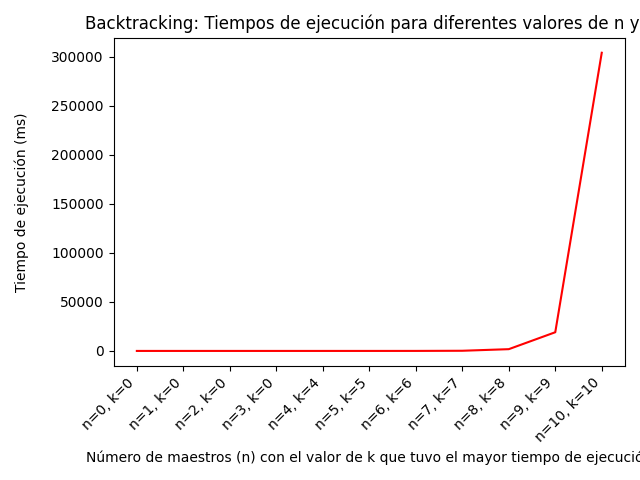
\includegraphics[scale=0.60]{images/graficoBacktracking.png}

Como podemos observar en la tendencia de la curva, el tiempo de ejecución aumenta exponencialmente con la cantidad de maestros $n$ y también depende de $k$. El tiempo más alto ocurre cuando $k$ se acerca a $n$, con $k < n$ (es lineal cuando $k = n$). Para valores pequeños de estas variables el algoritmo es relativamente rápido. Sin embargo, al incrementarlos no se vuelve práctico debido a que el tiempo no crece polinomialmente, sino exponencialmente.  Esto corrobora el análisis de la complejidad planteado previamente.

\subsubsection{Backtracking - greedy}
\label{sec:medidas-bt-greedy}
Procederemos a comparar esta versión del algoritmo de backtrcking con la anterior.

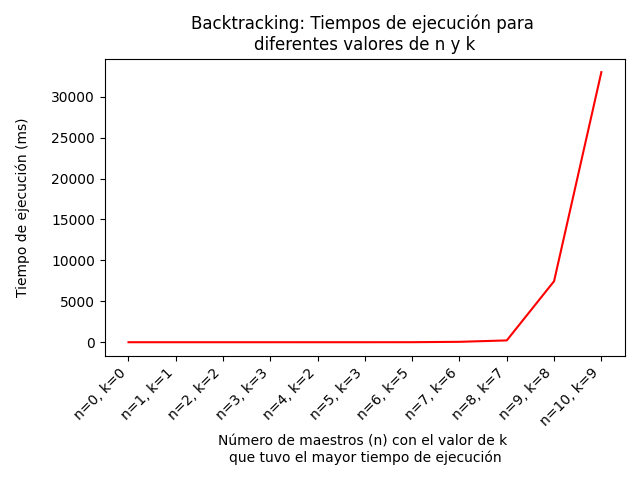
\includegraphics[scale=0.60]{images/graficoBacktrackingGreedy.png}

El gráfico evidencia una drástica disminución de los tiempos de ejecución, prácticamente a la mitad de los del otro algoritmo. 

Nuevamente podemos observar la tendecia exponencial de la curva, que comprueba nuestra justificación de la complejidad temporal.

\subsection{Algoritmo de programación lineal}
\subsection{Algoritmo de aproximación}


\section{Conclusión}


\end{document}
